\section{Coordinate Systems}
\label{sec:Coord}

	There are are number of different coordinate systems to be aware of and understand when dealing with the fitting, both in simulation and reconstruction. For obvious reasons, if the coordinate systems are not properly handled then the fitting will fail. I will summarize here the necessary information for the coordinate systems that are in use. (Other coordinate systems can be integrated and used if one wishes.)

	Before fitting, track information comes from the simulation geometry. See Figure \ref{fig:WorldCoordSys} for an overview of the simulation tracker geometry and some relevant coordinate system information. Some info from the figure caption is copied here. There is also some relevant information in the \hyperref[sec:RunGeane]{RunGeane} section. Three trackers live in the Geant4 world with Y vertical, where things like wire center coordinates are recorded as gm2geom::CoordSystem3Vectors which include a reference frame string as well as 3 coordinates. These CoordSystem3Vectors can be transformed from one to another using the transform(css, ``world'', true) function, where the first parameter is the coordinate system store, the second is the frame to be transformed to, and the third is a boolean value for whether momentum or position is being transformed. (Use ``true'' for momentum.)

	There are 3 specific coordinate systems defined in StrawTrackerCadMesh\_service.cc, GeaneTrackerWorld[0,12,18], where these are simple rotations around the vertical Y axis from the three tracker positions to a coodinate system where the tracking planes are parallel in X. These are rotations of -105.52, 74.48, and -15.52 degrees respectively where the numbers come from the geometric placement of the three trackers. (Note that the coordinate system with the tracking planes parallel in X is not actually centered at X = 0.) Only the first, GeaneTrackerWorld[0] is used when performing the error propagation stage of the fitting with the rotateArcTracker fcl parameter of the Arc service. All three are used however when transforming track information to be fitted, and when transforming the fitted track back to the world frame for the extrapolation. Again see Figure \ref{fig:WorldCoordSys} for more explanation on this. (There is also another general tracker frame with Z forward which is not in use because of the Z propagation bug.) 

	\begin{figure}[]
		\caption{Shown here is a picture of the 3 trackers in the world geometry in their approximate positions. First note the world coordinate system shown in the bottom left of the plot, where the origin lives at the center of the ring. Tracks are generated and read out from the trackers in their three world positions in the red boxes. Due to the reconstruction bug where tracks improperly reconstruct if their momenta is too aligned with the globabl Z axis, \href{http://gm2-docdb.fnal.gov:8080/cgi-bin/ShowDocument?docid=4567}{DocDB 4567}, the reconstruction rotates the entire arc including tracker 0 to the blue position, where planes are parallel in X, and the fitting is performed in this frame. Track parameters from the 3 separate positions are rotated to this reference frame by the amounts shown in the picture, fitted, and the fitted track at the end is rotated back. (For the parameters to fit, really just the wire center position is rotated, since the hit dcas are frame independent. The whole Geant geometry needs to be rotated however to include the proper energy loss when using the error propagation routines.)}
	\centering
	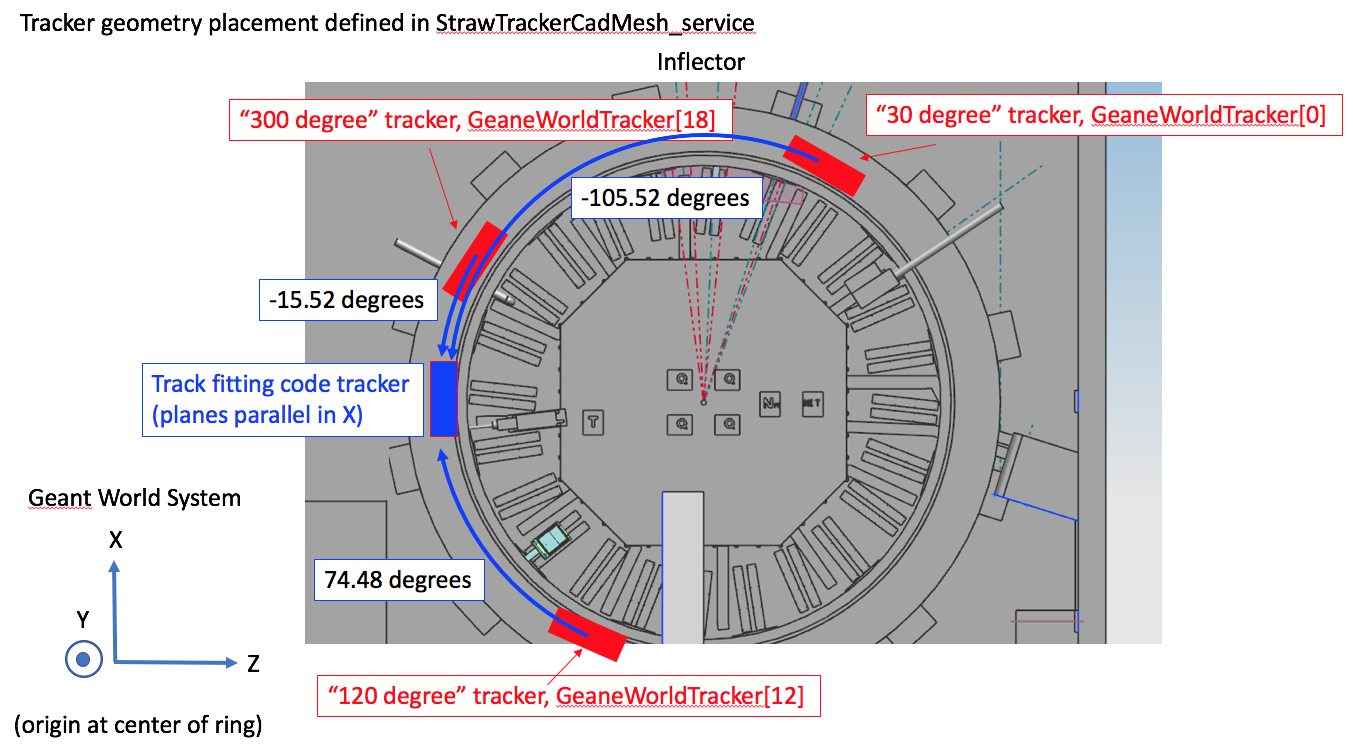
\includegraphics[width=1.0\textwidth]{WorldCoordSys}
	\label{fig:WorldCoordSys}
	\end{figure}


	For the fitting, there are a number of track parameterizations involved. I recommend reading the reference \cite{geanemanual} which has a quick intro on the different 5 parameter representations of a track, with 1 known parameter. For us this is the X parameter, which is given by virtue of knowing the placement of the trackers. There is also some good information in reference \cite{Lavezzi}. I will not describe here the exact meaning of these variables. There is the free system, 
		\begin{align}
			\frac{1}{p}, \lambda, \phi, y_{\perp}, z_{\perp},
		\end{align}
	and the surface system,
		\begin{align}
			\frac{1}{p}, \frac{py}{px}, \frac{pz}{px}, y, z.
		\end{align}
	(In the free system $y_{\perp}$ and $ z_{\perp}$ are defined with respect to the global Geant4 Z axis as defined in the references.) In the reconstruction, the Geane objects (matrices and parameter vectors) are defined and calculated in the Geant4 error propagation code in the free system. These objects are then transformed internally using Jacobians to the given XYZ surface system, where those Jacobians are defined in \cite{jacob}, and the tracker planes are parallel and staggered in X. Other surface systems can be given, but we just use XYZ where these are the global X, Y, and Z axes for simplicity. Finally, those objects are transformed to our most natural coordinate system,
		\begin{align}
			\frac{1}{p}, \frac{pu}{px}, \frac{pv}{px}, u, v,
		\end{align}
	the XUV system, using the simple Jacobian
		\begin{align}
			\begin{pmatrix}
				u \\
				v \\
			\end{pmatrix} =
			\begin{pmatrix}
				-\sin{\theta} & -\cos{\theta} \\
				\sin{\theta} & -\cos{\theta} \\
			\end{pmatrix}
			\begin{pmatrix}
				y \\
				z \\
			\end{pmatrix},
		\end{align}
	where $\theta$ is $7.5\degree$. The 5x5 transformation is just a 1 in the top left corner, and then this matrix in the remaining 2 diagonal blocks. (The reason this XUV system is not given as the initial surface system is because the Geant4 surface trajectory system must be defined in an orthogonal coordinate system.) These two surface systems can be seen in Figure \ref{fig:GeaneCoordSys}. It is in this coordinate system that the fitting is done as per the \hyperref[sec:Formalism]{Formalism} section.

	\begin{figure}[]
		\caption{This picture shows the coordinate system in which the the Geane track reconstruction is performed, in relation to the world coordinate system. The origin remains at the center of the ring, with the tracking planes parallel in X in the reconstruction, going forward in plane number. Y is vertically up, and Z is horizontally to the right. U and V are defined such that they have greater values with higher radii and increasing straw number.}
	\centering
	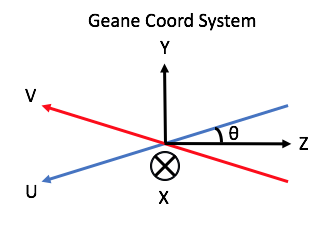
\includegraphics[width=0.4\textwidth]{GeaneCoordSys}
	\label{fig:GeaneCoordSys}
	\end{figure}

	
	Note that the coordinate system variables are switched or renamed among the different references and the Geant4 source code, so one needs to be very careful when trying to make sense of all of this. For instance, we use the XUV system when fitting, but the Geant4 source codes uses the variables UVW for a general surface system, and these variables are not equal. 
